\chapter{An\'alisis de resultados}

\label{Chapter4}

A lo largo del presente cap\'itulo, se analizar\'an los resultados obtenidos a partir de los experimentos planteados.
Se detallar\'an las m\'etricas obtenidas y los resultados de aplicar los modelos a los telegramas.

\section{An\'alisis de m\'etricas}

Los experimentos realizados arrojaron los resultados mostrados en el cuadro \ref{tab:metricas-experimentos}. Las
m\'etricas referidas a la capacidad de clasificaci\'on (Accuracy, $F_1$) son evaluadas sobre la partici\'on de test del
dataset de origen donde se conocen las etiquetas a ciencia cierta ($MNIST$). Por otro lado, las m\'etricas de
adaptaci\'on ($MMD$, Dist. $\mathcal{A}$) son evaluadas sobre los espacios latentes que los modelos generaron para las
particiones de test de ambos datasets. El mejor modelo es el que posea mejor capacidad de clasificaci\'on y de
adaptaci\'on.

% TODO: cambiar f1 por macro para que sea distinto a acc. que onda iou?
\begin{table}[H]
    \centering
    \begin{tabular}{cc|rrrr}
        \toprule
                                     &        & Acc.                                & $F_1$                               & $MMD$                               & Dist. $\mathcal{A}$                 \\
        AD                           & Modelo &                                     &                                     &                                     &                                     \\
        \midrule
        \multirow[c]{2}{*}{-}        & ResNet & {\footnotesize (2)} 0.9885          & {\footnotesize (2)} 0.9883          & 0.0632                              & 1.9306                              \\
                                     & LeNet  & 0.9811                              & 0.9810                              & 0.0469                              & 1.9515                              \\\hline
        \multirow[c]{2}{*}{DANN}     & ResNet & \textbf{{\footnotesize (1)} 0.9890} & \textbf{{\footnotesize (1)} 0.9890} & 0.1379                              & 1.9776                              \\
                                     & LeNet  & 0.9822                              & 0.9821                              & {\footnotesize (3)} 0.0090          & 1.6774                              \\\hline
        \multirow[c]{2}{*}{ADDA}     & ResNet & 0.9476                              & 0.9485                              & 0.0165                              & 1.8495                              \\
                                     & LeNet  & 0.9191                              & 0.9184                              & 0.0399                              & 1.8495                              \\\hline
        \multirow[c]{2}{*}{DANN+BSP} & ResNet & 0.9780                              & 0.9777                              & 0.0409                              & 1.7888                              \\
                                     & LeNet  & 0.9859                              & 0.9857                              & {\footnotesize (2)} 0.0051          & {\footnotesize (3)} 1.6369          \\\hline
        \multirow[c]{2}{*}{MDD}      & ResNet & {\footnotesize (3)} 0.9864          & {\footnotesize (3)} 0.9863          & 0.0615                              & 1.8987                              \\
                                     & LeNet  & 0.9856                              & 0.9854                              & 0.0399                              & 1.7468                              \\\hline
        \multirow[c]{2}{*}{AFN}      & ResNet & 0.9829                              & 0.9827                              & \textbf{{\footnotesize (1)} 0.0040} & \textbf{{\footnotesize (1)} 1.0886} \\
                                     & LeNet  & 0.9862                              & 0.9859                              & 0.0117                              & {\footnotesize (2)} 1.5747          \\

        \bottomrule
    \end{tabular}
    \caption{M\'etricas de los experimentos realizados. Entre par\'entesis se encuentra la posici\'on que ocupa dentro del top 3 de la columna.}
    \label{tab:metricas-experimentos}
\end{table}

Como era de esperarse, los modelos que fueron entrenados sin adaptaci\'on de dominio son los que mejores m\'etricas de
clasificaci\'on poseen. No obstante, sus valores de adaptaci\'on son los peores provocando que no puedan ser aplicados
en $TDS$.

El modelo que mejor combinaci\'on de clasificaci\'on y adaptaci\'on es la ResNet utilizando AFN. Cabe destacar que los
modelos LeNet entrenados con DANN y AFN obtuvieron buenas m\'etricas en general, lo que deja en evidencia que {\it no
        siempre un modelo m\'as complejo es mejor}.

Es posible aplicar los modelos sobre todos los telegramas y calcular el $IoU$ promedio por telegrama con el c\'alculo
descripto en el cap\'itulo \ref{Chapter3} y la cantidad de aciertos promedio por telegrama utilizando como etiquetas lo
transcripto en el centro de c\'omputo suponiendo que existen pocos errores en ellos.

\begin{table}[H]
    \centering
    \begin{tabular}{cc|rrr}
        \toprule
                                 &        & $IoU$ prom.     & \# aciertos prom. & \% aciertos prom. \\
        AD                       & Modelo &                 &                   &                   \\
        \midrule
        \multirow[c]{2}{*}{-}    & ResNet & 0.4494          & 4                 & 22\%              \\
                                 & LeNet  & 0.4715          & 6                 & 33\%              \\\hline
        \multirow[c]{2}{*}{MDD}  & ResNet & 0.5451          & 8                 & 44\%              \\
                                 & LeNet  & 0.5801          & 9                 & 50\%              \\\hline
        \multirow[c]{2}{*}{DANN} & ResNet & 0.6941          & 12                & 67\%              \\
                                 & LeNet  & 0.7024          & 12                & 67\%              \\\hline
        \multirow[c]{2}{*}{AFN}  & ResNet & \textbf{0.7486} & \textbf{13}       & \textbf{72\%}     \\
                                 & LeNet  & 0.6493          & 11                & 61\%              \\\hline
        \multirow[c]{2}{*}{ADDA} & ResNet & 0.6763          & 11                & 61\%              \\
                                 & LeNet  & 0.6406          & 10                & 56\%              \\
        \bottomrule
    \end{tabular}
    \caption{IoU promedio y cantidad promedio de aciertos al aplicar los modelos a cada telegrama.}
    \label{tab:iou-cant-aciertos-en-telegramas}
\end{table}

El cuadro \ref{tab:iou-cant-aciertos-en-telegramas} confirma la elecci\'on del mejor modelo realizada anteriormente.
Independientemente de qu\'e t\'ecnica de adaptaci\'on se utilice, todas presentan mejores porcentajes de aciertos
promedio que los modelos que fueron entrenados \'unicamente con $MNIST$.

\begin{figure}[H]
    \centering
    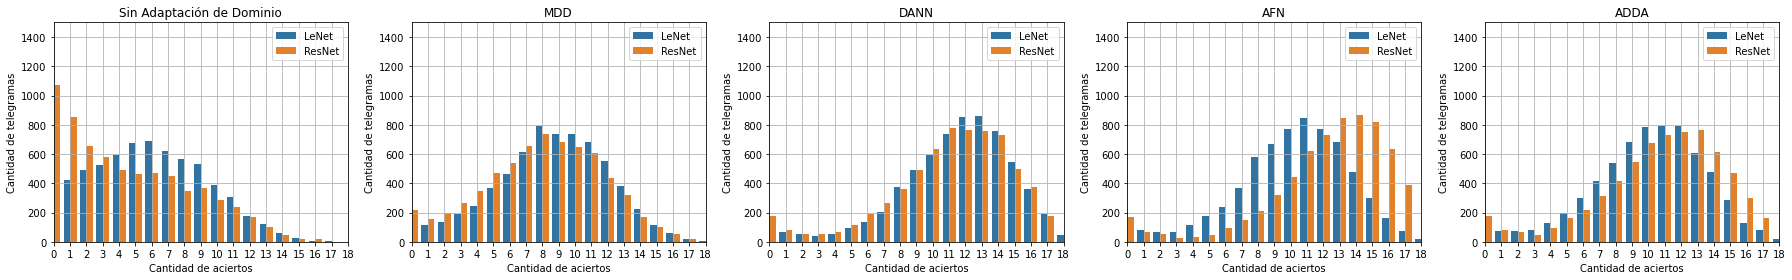
\includegraphics[width=1\textwidth]{chapter4/dist-aciertos.png}
    \caption{Distribuci\'on de aciertos de cantidad de votos por cada par t\'ecnica AD y modelo.}
    \label{fig:distribucion-aciertos}
\end{figure}

\section{Comparaci\'on de espacios latentes}

\lipsum[1]

\section{\'Analisis de errores}

Los errores de predicci\'on de los modelos pueden reflejarse en las distribuci\'on de la m\'etrica $IoU$ para cada uno
de ellos.

\begin{figure}[H]
    \centering
    \begin{subfigure}[h]{0.43\textwidth}
        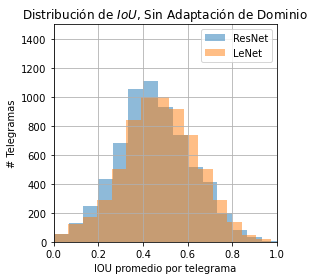
\includegraphics[height=1\textwidth]{chapter4/hist-iou-sin-da.png}
    \end{subfigure}
    \hfill
    \begin{subfigure}[h]{0.43\textwidth}
        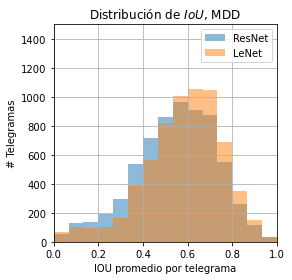
\includegraphics[height=1\textwidth]{chapter4/hist-iou-mdd.png}
    \end{subfigure}
    \hfill
    \begin{subfigure}[h]{0.43\textwidth}
        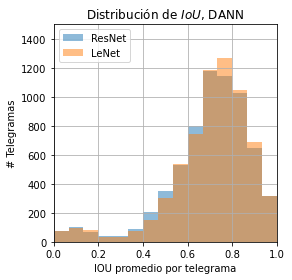
\includegraphics[height=1\textwidth]{chapter4/hist-iou-dann.png}
    \end{subfigure}
    \hfill
    \begin{subfigure}[h]{0.43\textwidth}
        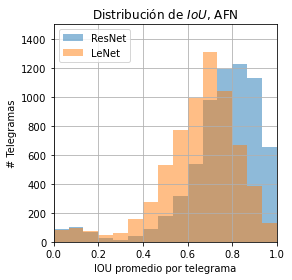
\includegraphics[height=1\textwidth]{chapter4/hist-iou-afn.png}
    \end{subfigure}
    \hfill
    \begin{subfigure}[h]{0.43\textwidth}
        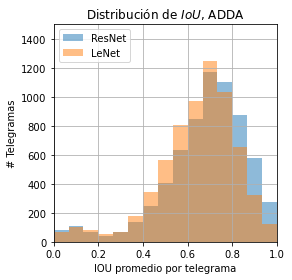
\includegraphics[height=1\textwidth]{chapter4/hist-iou-adda.png}
    \end{subfigure}

    \caption{Histogramas de la m\'etrica $IoU$ promedio por telegrama por cada par t\'ecnica AD y modelo.}
    \label{fig:histogramas-ious}
\end{figure}

Resulta interesante mencionar existen telegramas que son m\'as dif\'iciles de analizar que otros. Esto puede
evidenciarse en los histogramas de la figura \ref{fig:histogramas-ious} donde se pueden observar un conjunto de
observaciones que contienen valores entre [0, 0.2] en todos los experimentos realizados. Luego de analizar cada uno de
estos casos, se detectaron las siguientes situaciones:

\begin{itemize}
    \item Telegramas cargados de forma err\'ones: ver ejemplo en el anexo \ref{anexo:telegrama-erroneo}.
    \item Telegramas correctos pero por alguna cuesti\'on la l\'ogica de extracci\'on de d\'igitos no funciona correctamente: ver
          ejemplo en el anexo \ref{anexo:telegrama-numeros-juntos}.
    \item Telegramas donde existen otros caracteres distintos a n\'umeros: al ser un cuadro de texto libre sin formato, los jefes
          de mesa pueden escribir lo que deseen. Ver ejemplo en el anexo \ref{anexo:telegrama-erroneo-caracteres-especiales}
          donde se representa el $0$ a la izquierda con $X$.
    \item Telegramas de mesas donde la mayor cantidad de votos se las lleva un \'unico partido y completan los votos a la
          izquierda con $0$: al agregar los ceros a la izquierda, aumenta la probabilidad de que el modelo se equivoque con esos
          ceros que no aportan al n\'umero final. Ver ejemplo en el anexo \ref{anexo:telegrama-erroneo-muchos-ceros}.
\end{itemize}

En los primeros dos puntos se describen problemas problemas que fueron detectados en el proceso de ETL del cap\'itulo
\ref{Chapter3}. Estandarizar los telegramas agregando un casillero por cada d\'igito junto a mejorar el proceso de
extracci\'on de los mismos, supondr\'a una mejora considerable en las capacidades predictivas de los modelos.

El tercer punto presenta un problema dentro de la adaptaci\'on de dominio. La misma supone que, si bien los datasets de
origen y destino son diferentes pero representan lo mismo, debe existir la misma cantidad de clases entre origen y
destino. Al agregar uno o varios caracteres adicionales en $TDS$ (como es el ejemplo donde representaban el $0$ con una
$X$), se est\'a incumpliendo este supuesto.

El cuarto punto aumenta la probabilidad de error en los modelos debido a que el $0$ a la izquierda no aporta
significado alguno al n\'umero de la cantidad de votos que se desea predecir.

Estandarizar la carga de los telegramas por parte de los jefes de mesa mediante alguna capacitaci\'on permitir\'ia
reducir los errores de los puntos tres y cuatro en elecciones futuras.

